Various design choices lead to the definition of $\hat Y$ and its fitting. Given a causal model, these choices include:% the following:

First, $\hat Y$ is a function of a subset of $U \cup X$ and any
element of $X$ which is not a descendant of $A$ can be used in
building a fair classifier. If a strict subset of $U$ is used, the
causal model need not be fully specified: equation
$V_i = f_i(pa_i, U_{pa_i})$ can be substituted by a conditional
probability $p(V_i\ |\ pa_i, U_{pa_i}')$, where
$U_{pa_i}' \subset U_{pa_i}$ and
$p(V_i\ |\ pa_i, U_{pa_i}') = \int f_i(pa_i, U_{pa_i}) d U_{pa_i}''$,
where $U_{pa_i}'' \equiv U_{pa_i} \backslash U_{pa_i}'$. This
marginalization has implications in modeling discussed in the next
section.

Second, any random variable generated independently is trivially
counterfactually fair. However, we desire that $\hat Y$ is a {\it
  good} predictor, not something like tossing a coin. That is,
$\hat Y$ is to be understood as a parameterized function
$g_\theta(U, X)$ where $\theta$ is learned by minimizing the empiric
expected loss $E[l(Y, g_\theta(U, X))\ | X, A].$% , where the expectation
% is over $A \cup X \cup U \cup \{Y\}$.
For instance, $l(Y, g_\theta(U, X)) = (Y - g_\theta(U, X))^2$, or the
log-loss for Bernoulli classification.  In practice, the distribution
of $A \cup X \cup \{Y\}$ can be the empirical distribution as given by
some training data, while $p(U\ |\ X, A)$ comes from the estimated
causal model fit to the same training data. %  Markov chain Monte Carlo
% (MCMC) may be necessary to generate samples from this conditional,
% which means every training data point is replaced by a set of data
% points sharing the same $A \cup X \cup \{Y\}$ but with different
% replicates of $U$.
Any predictor can be used to learn $g_\theta(U, X)$
including random forests and neural networks.

\subsection{Limitations and a Guide to Model Building}
Causal modeling requires untestable assumptions. Experimental data can
sometimes be used to infer causal connections, but counterfactual
modeling requires functional
decompositions between background and endogenous variables.
Such decompositions are not
uniquely identifiable  with experimental data. As in several
matters of law and regulation, fairness at an individual level is a
counterfactual quantity and some level of assumptions
are unavoidable. As a guide for building fair predictive models, we
categorize assumptions by three levels of increasing strength.
%
\begin{itemize}
\item[L1] Given a causal DAG, build $\hat Y$
  using as covariates only the observable variables  not
  descendants of the protected attributes $A$. This
  requires information about the DAG, but no
  assumptions about structural equations or priors over background
  variables. %  Here
  % $\hat Y$ is not a function of $U$ but a function
  % of the maximal subset of $X$ that does not contain descendants of $A$;
\item[L2] This ignores much information, particularly if the protected
  attributes are typical demographic information such as race or sex, which are parents of many other variables. To
  include information from descendants of $A$, we postulate background
  latent variables that act as causes of observable variables, based
  on explicit domain knowledge and learning algorithms\footnote{In
    some domains, it is actually common to build a model entirely
    around latent constructs with few or no observable parents nor
    connections among observed variables \citep{bol:89}.}.  As these
  variables are not descendants of $A$, they can be used to fairly predict
  $\hat Y$.  Conditioning on descendants of $A$ propagates information
  from $X$ to them. This dependency of each $V_i$ on its parents can be
  probabilistic.% , instead of being given by a structural equation, as in the
  % previous section;
 \item[L3] In the above construction, the model factorizes as a
   general DAG, where each node follows a non-degenerate
   distribution given observed and latent variables. In the final
   level of assumptions, we remove all randomness from the conditional
   distributions to obtain a full decomposition $(U, V, F)$ of the
   model. % Default assumptions %partially independent of the domain,
   % might be invoked.
   For instance, the conditional distribution
   $p(V_i\ |\ V_1, \dots, V_{i - 1})$ can be treated as an additive
   error model, $V_i = f_i(V_1, \dots, V_{i - 1}) + e_i$
   \citep{peters:14}. The error term $e_i$  then becomes an input
   to $\hat Y$ after conditioning on the observable variables. This
   maximizes the information  extracted
   from a causal model by the fair predictor $\hat Y$.
\end{itemize}


\subsection{Special cases}
%
Consider the graph $A \rightarrow X \rightarrow Y$ (see
Figure~\ref{fig:ex1} (a)). In general, if $\hat Y$ is a function of
$X$ only, then $\hat Y$ need not obey demographic parity, i.e.
\begin{align}
  p(\hat Y\ |\ A = a) \neq p(\hat Y\ |\ A = a').\nonumber
\end{align}
If we postulate a
structural equation $X = \alpha A + e_X$, then given $A$ and $X$ we
can deduce $e_X$. If $\hat Y$ is a function of $e_X$ only and, by
assumption, $e_X$ is independent of $A$, then the assumptions imply
that $\hat Y$ will satisfy demographic parity, and that can be
falsified.

By way of contrast, if $e_X$ is not uniquely identifiable from the structural equation and $(A, X)$, then the distribution of $\hat Y$ depends on the value of $A$ as we marginalize $e_X$, and demographic parity will not follow. This leads to the following:

\begin{lem}
If all background variables $U' \subseteq U$ used in the definition of $\hat Y$ are determined from $(A, W)$, and all observable variables used in the definition of $\hat Y$ are independent of $A$ given $U'$, then $\hat Y$ satisfies demographic parity. % If the conditions fail, then $\hat Y$ will not satisfy demographic parity in general. 
\end{lem}
  
In one sense, Definition~\ref{eq:cf_definition} is a counterfactual
demographic parity condition, that can replace the
existing definition.

\begin{figure*}[!th]
\begin{center}
\vspace{-2ex}
\centerline{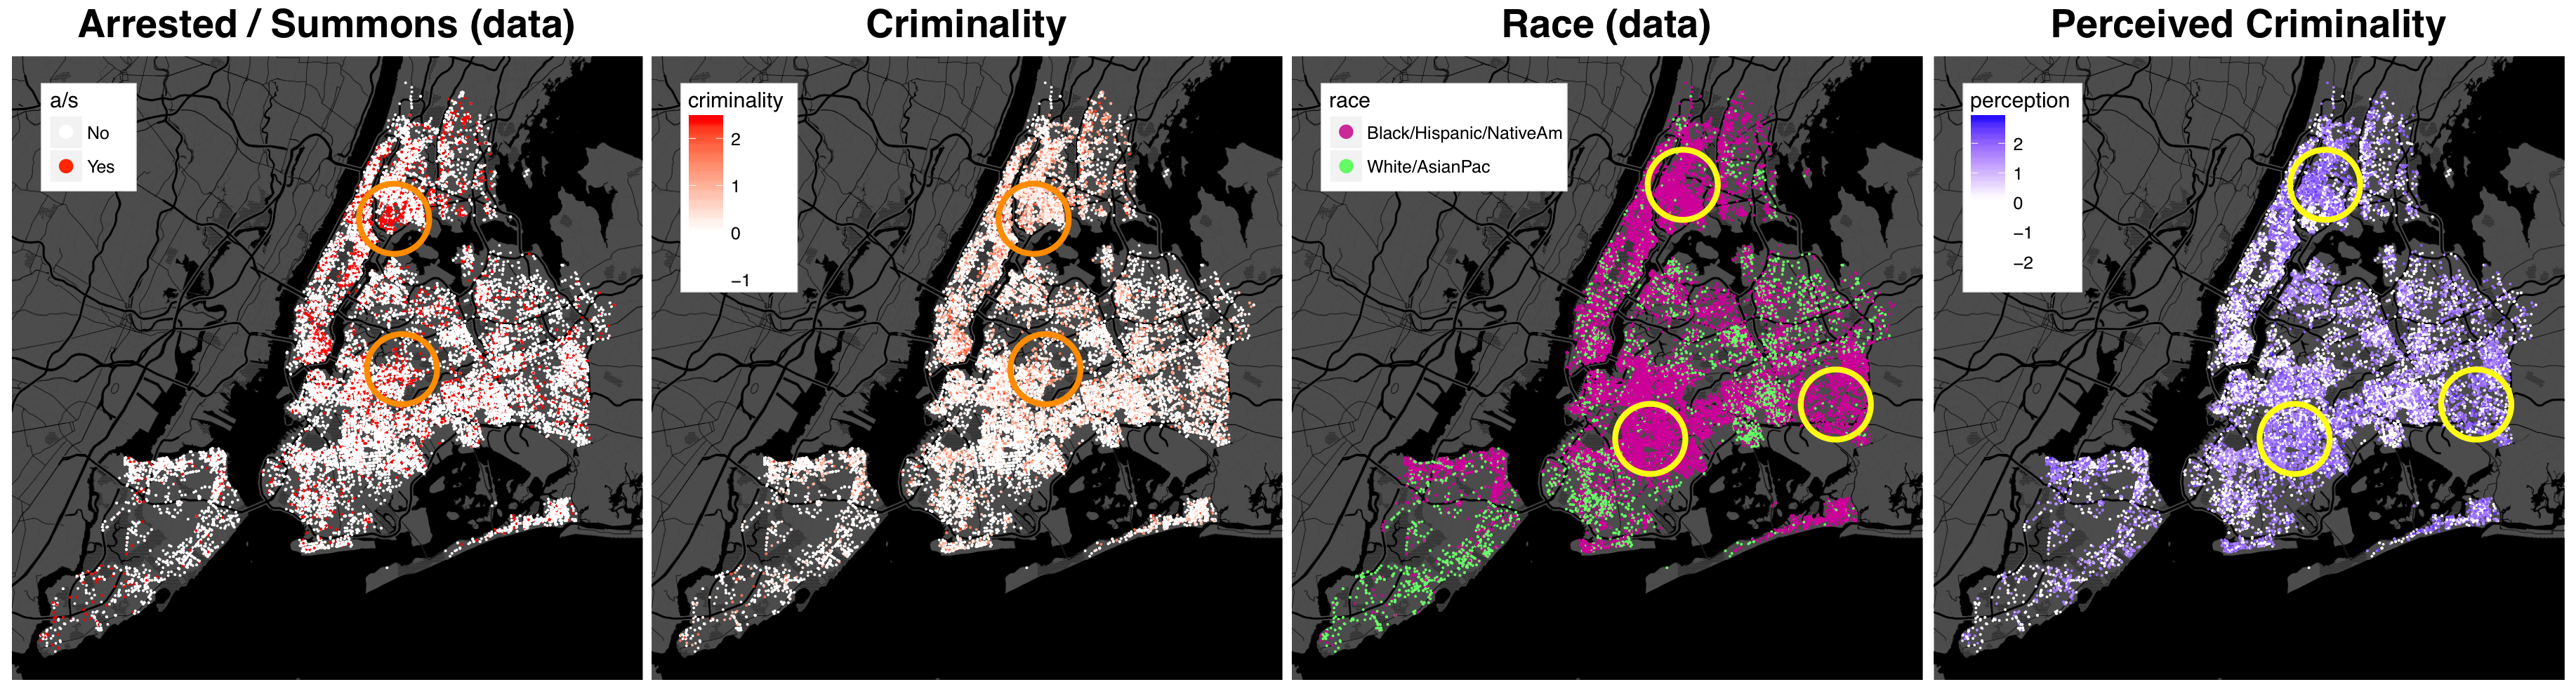
\includegraphics[width=\textwidth]{stop_and_frisk_graphs.png}}
\vspace{-2ex}
\caption{Understanding criminality. The above maps show the decomposition of stop and search data in New York into factors based on percieved criminality (a race dependent variable) and latent criminality (a race neutral measure). See \ref{sec:true-vs.-perceived}.     \label{figure.criminality}}
\vspace{-2ex}
\end{center}
\end{figure*}

We also advocate that counterfactual assumptions should underlie all approaches that separating the sources of variation of the data into ``fair'' and ``unfair'' components. As an example, \citet{louizos2015variational} explains the variability in $X$ from $A$ and an independent source $U$ following the DAG $A \rightarrow X \leftarrow U$. Since $U$ and $A$ are not independent given $X$ in this directed representation, a type of ``posterior regularization'' \citep{ganchev:10} is enforced such that a posterior $p_{fair}(U\ | A, X)$ is close to the model posterior $p(U\ |\ A, X)$ while having the property $p_{fair}(U\ | A = a, X) \approx p_{fair}(U\ | A = a', X)$. But this is neither necessary nor sufficient for counterfactual fairness if the model for $X$ given $A$ and $U$ is not justified by a causal mechanism. If it is, $p(U\ |\ A, X)$ is justified as distribution which we can use to marginalize $U$ in $p(\hat Y(U)\ |\ A, X)$. No posterior regularization is necessary.  Methods which estimate the relationship between $A$, $U$ and $X$ based on penalizing dependence measures between an estimated $U$ and $A$ are relevant in estimating a causal model such as the one described by \citet{mooij:09}, but this is motivated by a model in which $U$ is deterministically inferred from $A$ and $X$ by construction. Moreover, it is unclear in \citet{louizos2015variational} how the ideal label $Y$ is causally connected to $U$ and $A$, so that the semantics of the ``unfair''
components of $Y$ are left unexplained.


%%% Local Variables:
%%% mode: latex
%%% TeX-master: "ricardo_draft"
%%% End:
